\scanpage{6}
\mspage{\textcircled{2}}
\[
\underbrace{\underline{\mathrm{Hom}}_k^!(Q^{\unsure{\&}\circ},M)}_{\mathcal Q_M}
\simeq
\underbrace{\underline{\mathrm{Hom}}_{k!}(P^{\unsure{\&}},M)}_{\mathcal P^M}
\qquad\text{si }M\text{ $k$-add. st.\unsure{ble} par les deux types de lim}
\]
Sur $\mathcal P_M^{\deleted{\unsure{\&}}}\xrightarrow{\simeq}
\underline{\mathrm{Hom}}_k(P^\circ,M)$
\[
\mathcal Q=\mathcal P^\vee\text{ opère par }(F,L')\longmapsto F*_kL'
\]
\margin{$\overbrace{\mathcal P_M^{\deleted{\unsure{\&}}}\times\mathcal Q}^{P_M^{\unsure{\&}}\times Q^{\unsure{\&}}}\longrightarrow M$}
\[
\mathcal P\text{ opère par }(L,F)\longmapsto\underline{\mathrm{Hom}}_k(L,F)
\]
\margin{$\underbrace{\mathcal P\times\mathcal P_M^{\unsure{!}}}_{P^{\unsure{\&}}\times P_M^{\unsure{\&}}}\longrightarrow M$}
On a
\[
(\underbrace{F*_kL'}_{P,M})^\circ\simeq\deleted{\unsure{E}}
\underbrace{\underline{\mathrm{Hom}}_k(L',F^\circ)}_{Q,M^\circ}
\]
\[
(\overbrace{\underline{\mathrm{Hom}}_k(L,F)}^{P,M})^\circ
\simeq\overbrace{F^\circ*L}^{Q,M^\circ}
\qquad\deleted{\unsure{\underbrace{\phantom{Hom}}}}
\]
\deleted{$\unsure{\mathcal Q^\circ\simeq\mathcal P}$}
\figure{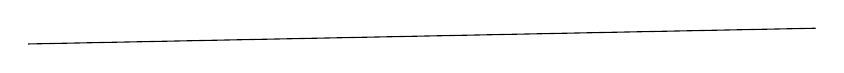
\begin{tikzpicture}\draw (0,0)--(10,.2);\end{tikzpicture}}

Soient $P,Q$ $k$-additives, on définit $P\otimes_kQ$ et
$\underbrace{P\times Q\unsure{-|\longrightarrow}P\otimes_kQ}_{k\text{-biadditive}}$
de façon 2-universelle :
\[
\underline{\mathrm{Hom}}_k(P\otimes_kQ,M)\simeq\operatorname{Bil}_k(P,Q;M)
\qquad\text{tout }M\text{ $k$-additive}
\]
Construction explicite par familles finies d'objets de $P\times Q$
\[
\unsure{\zeta|\xi}=\bigoplus_{i\in I}a_i\otimes_k b_i
\]
avec, pour
\[
\unsure{\zeta|\xi}'=\bigoplus_{j\in\unsure{J|I}}a'_j\otimes_k b'_j
\]
\[
\mathrm{Hom}(\unsure{\zeta|\xi},\unsure{\zeta|\xi}')=
\prod_{I\times J}\mathrm{Hom}(a_i,a'_j)\otimes_k\mathrm{Hom}(b_i,\unsure{b'_j|b_j})
\]
À retenir

 a) Si $P,Q$ petites, $P\otimes_kQ$ est petite
\[
\text{b)}\quad
\mathrm{Hom}_{P\otimes_kQ}(a\otimes_kb,a'\otimes_kb')
\xleftarrow{\sim}\mathrm{Hom}_P(a,a')\otimes_k\mathrm{Hom}_Q(b,b')
\]
On en conclut que le foncteur \inserted{can} (pl. fid !)
% archive foliation: 5
